\section{Statische Programmanalyse \& Metriken}
Statische Codeanalyse verlangt ein stures, monotones Anwenden von relativ ein-
fachen Regeln auf oft umfangreichen Code. Diese Aufgabe erfordert keinerlei Kreativität aber eine sehr große Übersicht und Kontrolle. ... Statische Codeanalyse ist daher prädestiniert zur Automatisierung durch Werkzeuge. Ich empfehle Ihnen, diese Techniken entweder werkzeuggestützt oder gar nicht einzusetzen.

\subsection{Einleitung}
\begin{itemize}
	\item Oft (fast immer) finden sich \textbf{80\% aller Probleme} mit einem Softwaresystem in 20\% des entwickelten Codes. 
	\item Die statische Programmanalyse versucht meist werkzeuggestützt frühzeitig die \textbf{problematischen 20\%} eines Softwaresystems zu finden.
	\item Statische Analyseverfahren identifizieren Programmteile von \textbf{fragwürdiger Qualität} und liefern damit Hinweise auf potentielle Fehlerstellen.
	\item Statische Analyseverfahren \textbf{versuchen} die Qualität von Software zu \textbf{messen}, können deshalb zur Festlegung von Qualitätsmaßstäben eingesetzt werden.
	\item Die statische Programmanalyse setzt \textbf{keine vollständig ausführbaren} Programme voraus.
	\item Die statische Programmanalyse kann also \textbf{frühzeitig} bei der Neuentwicklung und kontinuierlich bei der Wartung eines Softwaresystems eingesetzt werden.
\end{itemize}

\paragraph{Analytisches Qualitätsmanagement zur Fehleridentifikation:}
\begin{itemize}
	\item \textbf{analysierende Verfahren:} \\
	der ''Prüfling'' (Programm, Modell, Dokumentation) wird von Menschen oder Werkzeugen auf Vorhandensein/Abwesenheit von Eigenschaften untersucht
	\begin{itemize}
		\item \textbf{Review} (Inspektion, Walkthrough): Prüfung durch (Gruppe v.) Menschen
		\item \textbf{statische Analyse}: werkzeuggestützte Ermittlung von ''Anomalien''
		\item \textbf{(formale) Verifikation}: werkzeuggestützter Beweis von Eigenschaften 
	\end{itemize}
	\item \textbf{testende Verfahren:} \\
	der ''Prüfling'' wird mit konkreten oder abstrakten Eingabewerten auf einem Rechner ausgeführt
	\begin{itemize}
		\item \textbf{dynamischer Test}: ''normale'' Ausführung mit ganz konkreten Eingaben
		\item \textbf{[symbolischer Test}: Ausführung mit symbolischen Eingaben (die oft unendliche Mengen möglicher konkreter Eingaben repräsentieren)]
	\end{itemize}
\end{itemize}

\paragraph{Arten der Programmanalyse}
\begin{itemize}
	\item \textbf{Visualisierung von Programmstrukturen}: unästhetisches Layout liefert Hinweise auf sanierungsbedürftige Teilsysteme
	\item \textbf{manuelle Reviews}: organisiertes Durchlesen u. Diskutieren von Entwicklungsdokumenten durch Menschen
	\item \textbf{Compilerprüfungen}: Syntaxprüfungen, Typprüfungen, ...  
	\item \textbf{Programmverifikation und symbolische Ausführung}: Beweis der Korrektheit eines Programms mit Logikkalkül oder anderen mathematischen Mitteln
	\item \textbf{Stilanalysen}: Programmierkonventionen für Programmiersprachen
	\item \textbf{Kontroll- und Datenflussanalysen}: die Programmstruktur wird untersucht, um potentielle Zugriffe auf undefinierte Variablen, möglicherweise nie ausgeführten Code, etc. zu entdecken.
	\item \textbf{Metriken}: Programmeigenschaften werden gemessen und als Zahl repräsentiert - in der Hoffnung, dass kausaler Zusammenhang zwischen Softwarequalität (z.B. Fehlerzahl) und berechneter Maßzahl besteht.
\end{itemize}

\subsection{Softwarearchitekturen und -visualisierung}
Große Systeme sind immer in Subsysteme gegliedert, von denen jedes eine Anzahl von Diensten bereitstellt. Der fundamentale Prozess zur Definition dieser Subsysteme und zur Errichtung eines Rahmenwerkes für die Steuerung und Kommunikation dieser Subsysteme wird \textbf{Entwurf der Architektur} ... genannt.

\paragraph{Begriffe nach Sommerville:}
\begin{itemize}
	\item Ein \textbf{Softwaresystem} besteht aus Teilsystemen, die zusammengehörige Gruppen von Diensten anbieten und möglichst unabhängig voneinander realisiert sind.
	\item Ein \textbf{Teilsystem} kann wiederum aus Teilsystemen aufgebaut werden, die aus Moduln (Paketen) bestehen.
	\item Ein \textbf{Modul} (Paket) bietet über seine Schnittstelle Dienste an und benutzt (importiert) zu ihrer Realisierung Dienste anderer Module (Pakete).
	\item Ein Modul fasst ''verwandte'' Prozeduren, \textbf{Klassen}, ... zusammen.
\end{itemize}

\paragraph{Softwarearchitekturen sind mehr als Teilsysteme und Module:}
\begin{itemize}
	\item In den 80er Jahren wurden Programmarchitekturen mit sogenannten ''Module Interconnection Languages (\textbf{MIL})'' definiert, die nur Module und Import-Beziehungen kennen.
	\item Seit den 90er Jahren werden auch ''Architecture Description Languages'' (\textbf{ADLs}) eingesetzt, die Komponenten mit Eingängen und Ausgängen und Verbindungen dazwischen verwenden (siehe Vorlesung „Echtzeitsysteme“);
	\item Heute verwendet man einen noch umfassenderen Architekturbegriff; in ''Software Engineering I'' werden folgende \textbf{Architektursichten} im Zusammenhang mit der ''Unified Modeling Language'' (\textbf{UML}) eingeführt:
	\begin{itemize}
		\item Teilsystem-Sicht (Paketdiagramme)
		\item Struktur-Sicht (Klassendiagramme, Kollaborationsdiagramme)
		\item Kontrollfluss-Sicht (Aktivitätsdiagramme, ... )
		\item Datenfluss-Sicht (Aktivitätsdiagramme, ... )
	\end{itemize}
\end{itemize}

\paragraph{Statische Visualisierung von Programmstruktur mit CrocoCosmos:}
\begin{itemize}
	\item grafische Darstellung eines Rahmenwerks für interaktive Anwendungen
	\item Klassen eines Teilsystems besitzen dieselbe Farbe, Beziehungen zwischen Klassen (aus Gründen der Übersichtlichkeit weggelasssen)
\end{itemize}
\begin{figure}[h]
	\centering
	\caption{Grafische Darstellung eines Rahmenwerks für interaktive Anwendungen}
	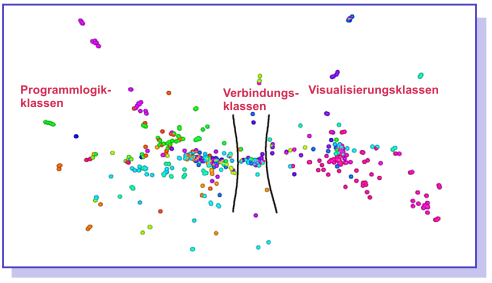
\includegraphics[width=0.85\textwidth]{3_1_1}
\end{figure}
\begin{figure}[h]
\centering
\caption{Ausschnitte der Programmlogik}
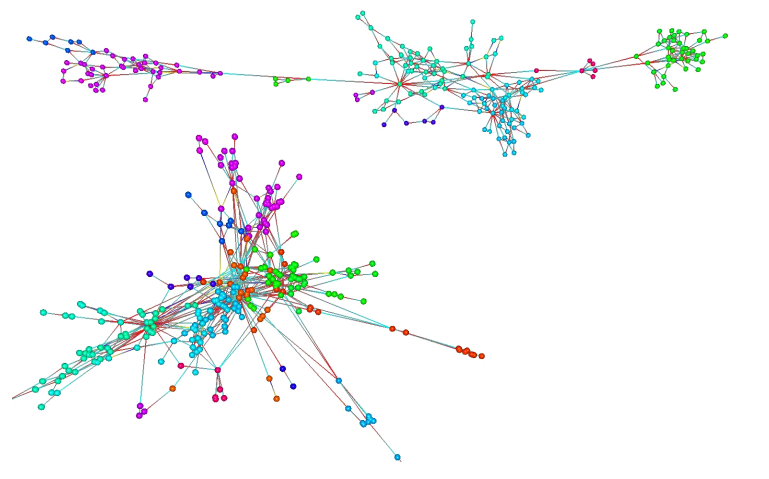
\includegraphics[width=0.85\textwidth]{3_1_2}
\end{figure}

\paragraph{Programmvisualisierung mit Doxygen und Graphviz:}
\begin{itemize}
	\item Doxygen generiert Programmdokumentation, Architekturdiagramme, etc.
	\item Graphviz (dot) ist ein Hilfsprogramm für Layoutberechnung;
\end{itemize}

\subsection{Strukturierte Gruppenprüfungen (Reviews)}
Systematische Verfahren zur gemeinsamen „Durchsicht“ von Dokumenten (wie z.B. erstellte UML-Modelle, implementierten Klassen, … ):
\begin{itemize}
	\item \textbf{Inspektion}: stark formalisiertes Verfahren bei dem Dokument nach genau festgelegter Vorgehensweise durch Gutachterteam untersucht wird
	\item \textbf{Technisches Review}: weniger formale manuelle Prüfmethode; weniger Aufwand als bei Inspektion, ähnlicher Nutzen
	\item \textbf{Informelles Review (Walkthrough)}: unstrukturiertere Vorgehensweise; Autor des Dokuments liest vor, Gutachter stellen spontane Fragen
	\item \textbf{Pair Programming}: Programm wird von vornherein zu zweit erstellt
\end{itemize}
Empirische Ergebnisse zu Programminspektion:
\begin{itemize}
\item Prüfaufwand liegt bei ca. 15 bis 20\% des Erstellungsaufwandes
\item 60 bis 70\% der Fehler in einem Dokument können gefunden werden
\item Nettonutzen: 20\% Ersparnis bei Entwicklung, 30\% bei Wartung
\end{itemize}

\paragraph{Psychologische Probleme bei Reviews:}
\begin{itemize}
	\item \textbf{-}: Entwickler sind in aller Regel von der Korrektheit der erzeugten Komponenten überzeugt (ihre Komponenten werden höchstens falsch benutzt)
	\item \textbf{-}: Komponententest wird als lästige Pflicht aufgefasst, die
	\begin{itemize}
		\item Folgearbeiten mit sich bringt (Fehlerbeseitigung) 
		\item Glauben in die eigene Unfehlbarkeit erschüttert
	\end{itemize}
	\item \textbf{-}: Entwickler will eigene Fehler (unbewusst) nicht finden und kann sie auch oft nicht finden (da ggf. sein Testcode von denselben falschen Annahmen ausgeht)
	\item \textbf{-}: Fehlersuche durch getrennte Testabteilung ist noch ärgerlicher (die sind zu doof zum Entwickeln und weisen mir permanent meine Fehlbarkeit nach)
	\item \textbf{+}: Inspektion und seine Varianten sind u.a. ein Versuch, diese psychologischen Probleme in den Griff zu bekommen
	\item \textbf{+}: Rolle des Moderators ist von entscheidender Bedeutung für konstruktiven Verlauf von Inspektionen
\end{itemize}

\paragraph{Vorgehensweise bei der Inspektion}
\begin{itemize}
	\item \textbf{Inspektionsteam} besteht aus Moderator, Autor (passiv), Gutachter(n), Protokollführer und ggf. Vorleser (nicht dabei sind Vorgesetzte des Autors / Manager)
	\item \textbf{Gutachter} sind in aller Regel selbst (in anderen Projekten) Entwickler
	\item Inspektion \textbf{überprüft}, ob:
	\begin{itemize}
		\item Dokument Spezifikation erfüllt (Implementierung konsistent zu Modell)
		\item für Dokumenterstellung vorgeschriebene Standards eingehalten wurden
	\end{itemize}
	\item Inspektion hat \textbf{nicht zum Ziel}:
	\begin{itemize}
		\item zu untersuchen, wie entdeckte Fehler behoben werden können
		\item Beurteilung der Fähigkeiten des Autors
		\item lange Diskussion, ob ein entdeckter Fehler tatsächlich ein Fehler ist
	\end{itemize}
	\item \textbf{Inspektionsergebnis:}
	\begin{itemize}
		\item formalisiertes Inspektionsprotokoll mit Fehlerklassifizierung
		\item Fehlerstatistiken zur Verbesserung des Entwicklungsprozesses
	\end{itemize}
\end{itemize}

\paragraph{Ablauf einer Inspektion:}
\begin{itemize}
	\item \textbf{Planung} des gesamten Verfahrens durch Management und Moderator
	\item \textbf{Auslösung} der Inspektion durch Autor eines Dokumentes (z.B. durch Freigabe)
	\item \textbf{Eingangsprüfung} durch Moderator (bei vielen offensichtlichen Fehlern wird das Dokument sofort zurückgewiesen) 
	\item \textbf{Einführungssitzung}, bei der Prüfling den Gutachtern vorgestellt wird
	\item \textbf{Individualuntersuchung} des Prüflings (Ausschnitt) durch Gutachter (zur \textbf{Vorbereitung} auf gemeinsame Sitzung) anhand ausgeteilter Referenzdokumente 
	\item auf \textbf{Inspektionssitzung} werden Prüfergebnisse mitgeteilt und protokolliert sowie Prüfling gemeinsam untersucht
	\item \textbf{Nachbereitung} der Sitzung und  \textbf{Freigabe} des Prüflings durch Moderator (oder Rückgabe zur Überarbeitung)
\end{itemize}

\paragraph{Technisches Review (abgeschwächte Form der Inspektion):}
\begin{itemize}
	\item Prozessverbesserung und Erstellung von Statistiken steht nicht im Vordergrund
	\item Moderator gibt Prüfling nicht frei, sondern nur Empfehlung an Manager
	\item kein formaler Inspektionsplan mit wohldefinierten Inspektionsregeln
	\item Ggf. auch Diskussion alternativer Realisierungsansätze
\end{itemize}

\paragraph{Informelles Review (Walkthrough):}
\begin{itemize}
	\item Autor des Prüflings liest ihn vor (ablauforientiert im Falle von Software) 
	\item Gutachter versuchen beim Vorlesen ohne weitere Vorbereitung Fehler zu finden
	\item Autor entscheidet selbst über weitere Vorgehensweise
	\item Zielsetzungen:
	\begin{itemize}
		\item Fehler/Probleme im Prüfling identifizieren
		\item Ausbildung/Einarbeitung von Mitarbeitern
	\end{itemize}
\end{itemize}

\subsection{Kontroll- und Datenflussorientierte Analysen}
Der Kontrollflussgraph ist ... eine häufig verwendete Methode zur Darstellung von Programmen. ... Die Verarbeitungssteuerung übernehmen die Kontrollstrukturen der Software unter Nutzung der Datenwerte. Eingabedaten werden gelesen, um Zwischenergebnisse zu bestimmen, die in den Speicher geschrieben werden, ... . Die Daten „fließen“ quasi durch die Software; von Eingaben zu Ausgaben.
\\
Ein \textbf{gerichteter Graph} G ist ein Tupel (N,E) mit N, eine Menge von \textbf{Knoten} (Nodes) und E einer Menge gerichteter \textbf{Kanten} (Edges).

\paragraph{Kontrollflussgraph - formale Definition:}
Ein \textbf{Kontrollflussgraph} eines Programms (Prozedur) ist ein Gerichteter Graph $ G = (N, E, n_{start}, n_{final})$ mit 
\begin{itemize}
	\item $N$ ist die Menge der \textbf{Anweisungen} (Knoten) eines Programms
	\item $E \subseteq N x N$ ist die Menge der \textbf{Zweige} (Kanten) zwischen den Anweisungen des Programms
	\item $n_{start} \epsilon N $ ist der \textbf{Startknoten} des Programms
	\item $n_{end} \epsilon N $ ist der \textbf{Endknoten} des Programms
\end{itemize}
Es gilt für den Kontrollflussgraphen:
\begin{itemize}
	\item keine in den Startknoten einlaufenden Kanten
	\item keine aus dem Endknoten auslaufenden Kanten
\end{itemize}
Manchmal wird zusätzlich gefordert, dass Kontrollflussgraphen zusammenhängen sind:
\begin{itemize}
	\item es gibt einen Pfad von $n_{start}$ nach $n$
	\item es gibt einen Pfad von $n$ nach $n{final}$
\end{itemize}

\paragraph{Pfade im Kontrollflussgraphen - formale Definition}
Ein \textbf{Pfad der Länge k} in einem Kontrollflussgraphen ist eine Knotenfolge.
\\
Ein \textbf{zyklenfreier Pfad} enthält keinen Knoten zweimal.
\\
Ein \textbf{Zyklus} ist ein Pfad mit $n_{1} = n_{k}$.

\paragraph{Kontrollflussgraphsegmente - formale Definition}
Ein \textbf{Segment} oder \textbf{Block} eines Kontrollflussgraphen ist ein Knoten $s$, der einen Teilgraph ersetzt, der aus einem zyklenfreien Pfad besteht mit genau einer auslaufenden und einer einlaufenden Kante.

\paragraph{Datenflussattribute eines Kontrollflussgraphen}
Die Anweisungen eines Kontrollflussgraphen besitzen Datenflussattribute, die den Zugriffen auf Variable (Parameter,...) in den Anweisungen entsprechen:
\begin{itemize}
	\item $n \epsilon N$ besitzt das Attribut \textbf{def(v)} oder kurz \textbf{d(v)}, falls $n$ eine Zuweisung an $v$ enthält (Wert von $v$ definiert); \\
	gilt auch für Eingabeparameter bei $n_{start}$
	\item $n \epsilon N$ besitzt das Attribut \textbf{c-use(v)} oder kurz \textbf{c(v)}, falls $n$ eine Berechnung mit Zugriff auf $v$ enthält (c=compute); \\
	implizite Zuweisung an Ausgabeparameter am Ende ist auch c-use
	\item $n \epsilon N$ besitzt das Attribut \textbf{p-use(v)} oder kurz \textbf{p(v)}, falls n eine Fallentscheidung mit Zugriff auf $v$ enthält (p=predicative)
	\item $n \epsilon N$ besitzt das Attribut \textbf{r(v)}, falls es das Attribut \textbf{c(v)} oder \textbf{p(v)} besitzt, also lesend auf $v$ zugreift (r=reference); \\
	dient nur der Zusammenfassung von c(v) und p(v), wenn der Unterschied c/p irrelevant ist
	\item $n \epsilon N$ besitzt das Attribut \textbf{u(v)}, falls $v$ in dieser Anweisung (noch) keinen definierten Wert (mehr) besitzen kann
\end{itemize}

\paragraph{Kontrollflussgraphsegmente mit Datenflussattributen}
\begin{itemize}
	\item Sei s ein Kontrollflussgraphsegment mit Pfad $n_{start} = n_{1}, ..., n_{k} = n_{final}$ und $attr(n_{i})$ die Sequenz der Datenflussattribute der $n_{i}$. Dann ist $attr(s) := attr(n_{1}, ..., attr/n_{k})$ die Konkatenierung der Datenflussattributsequenzen von $n_1$ bis $n_k$
	\item Ein Knoten n mit einer Sequenz von Datenflussattributen $attr(n) := attr_{1}, ..., attr_{k}$ ist immer eine abkürzende Schreibweise für einen Pfad von Knoten $n_1, ..., n_{k}$, sodass jeder Knoten $n_{i}$ genau einen Datenflussattribut besitzt $attr(n_{i}) := attr_{i}$
	\item Allen folgenden Definitionen liegt immer ein ''segmentfreier'' Kontrollflussgraph zugrunde, in dem jeder Knoten genau ein Datenflussattribut besitzt
\end{itemize}

\paragraph{Inout-Parameterdiskussion und Aufruf von Prozeduren}
Die meisten Programmiersprachen erlauben \textbf{nicht} die Auszeichnung von Variablen, die reinen Ausgabeparameter-Charakter besitzen; in Pascal/Modula gibt es nur mit VAR gekennzeichnete \textbf{Inout-Parameter}, in Sprachen wie C oder C++ hat man nur die Möglichkeit, out-Parameter als Zeiger/Referenzen auf Variable/Objekte zu simulieren.
\\
\\
Für solche Parameter mit Ein- und Ausgabecharakter müssen wir wie folgt vorgehen:
\begin{itemize}
	\item Deklaration der Prozedur countVowels(IN s:...; INOUT count: ...): für $n_{start}$ wird d(count) sowie d(s) angenommen, da beide Variablen bei der Übergabe einen definierten Wert haben sollten. \\
	Für $n_{final}$ wird c(count) angenommen, da am Ende der Prozedur der Wert von count durch versteckte Zuweisung an Aufrufstelle übergeben wird.
	\item Aufruf der Prozedur countVowels(aSentence, aCounter): \\
	es wird c(aSentence) und c(aCounter) in normaler Anweisung oder p(aSentence) und p(aCounter) in Prädikat gefolgt von d(aCounter) angenommen, da beim Aufruf versteckte Zuweisungen die Werte von aSentence und aCounter an die Parameter s und count zuweisen
\end{itemize}

\paragraph{Felder, globale Variablen und Strukturen}
\begin{itemize}
	\item Zugriff auf \textbf{globale Variablen} in einer Prozedur (Methode): werden bei Ein- und Austritt aus der Prozedur ignoriert und ansonsten wie lokale Variablen behandelt
	\item Zugriff auf \textbf{Felder (Arrays)}:
	\begin{itemize}
		\item anArray[index] := ... wird als r(index) und d(anArray) gewertet
		\item .. := .. anArray[index] ... wird als r(index) und r(anArray) gewertet
	\end{itemize}
	\item Zugriff auf \textbf{Strukturen}: wenn notwendig, können die Bestandteile (Variablen) einer Struktur als einzelne Variablen behandelt werden
\end{itemize}

\paragraph{Datenflussgraph - formale Definition}
Ein \textbf{Datenflussgraph} $D = (V_{d}, E_{d})$ zu einem Kontrollflussgraphen G eines Programms besteht aus
\begin{itemize}
	\item einer Menge von Knoten $V_{d}$ für alle Anweisungen V des Programms
	\item einer Menge von \textbf{Datenflusskanten} $E_{d}$: \\
	$ (n_{1}, n_{2}) \epsilon E_{d} $ genau dann, wenn es einen Pfad p im Kontrollflussgraphen G von $n_{1}$ nach $n_{2}$ gibt, sodass für eine Variable/Parameter v gilt:
	\begin{enumerate}
		\item d(v) für $n_{1}$: Anweisung $n_{1}$ definiert Wert für v
		\item r(v) für $n_{2}$: Anweisung $n_{2}$ benutzt Wert von v
		\item für alle Anweisungen n auf Pfad p (ohne $n_{1}$), gilt nicht d(v) für n: \\
		n ändert also nicht den bei $n_{1}$ festgelegten Wert von v
	\end{enumerate}
\end{itemize}
Die Kanten des Datenflussgraphen verbinden also Zuweisungen an Variablen oder Parameter mit den Anweisungen, in denen die zugewiesenen Werte benutzt werden.

\paragraph{Programm-Slices zur Fehlersuche und Änderungsfolgeschätzung}
Ein \textbf{Abhängigkeitsgraph} $A = (N_{a}, E_{a})$ eines Programms ist ein gerichteter Graph, der
\begin{itemize}
	\item alle Knoten und Kanten des Datenflussgraphen enthält (ohne Zusammenfassung von Teilgraphen zu Segmenten) sowie zusätzlich
	\item Kanten (des Kontrollflussgraphen) von allen Bedingungen zu direkt kontrollierten Anweisungen (das sind die Anweisungen, deren Ausführung von der Auswertung des betrachteten Bedingung abhängt).
\end{itemize}
Es gibt zwei Arten von Ausschnitten (Slices) eines Abhängigkeitsgraphen A:
\begin{itemize}
	\item \textbf{Vorwärts-Slice} für Knoten $n \epsilon N_{a}$ mit Datenflussattribut d(v): \\
	alle Pfade in A, die von Knoten n ausgehen, der Variable v definiert (der Slice-Graph enthält alle Knoten und Kanten der Pfade)
	\begin{itemize}
		\item Ein Vorwärts-Slice zu einer Anweisung n, die einer Variable v einen Wert zuweist, bestimmt alle die Stellen eines Programms, die von einer Änderung des zugewiesenen Wertes (Berechnungsvorschrift) betroffen sein könnten.
		\item Ein Vorwärts-Slice dient der Abschätzung von Folgen einer Programmänderung.
	\end{itemize}
	\item \textbf{Rückwärts-Slice} für Knoten $n \epsilon N_{a}$ mit Datenflussattribut r(v): \\
	alle Pfade in A, die in Knoten n einlaufen, der Variable v referenziert (der Slice-Graph enthält alle Knoten und Kanten der Pfade)
	\begin{itemize}
		\item Ein \textbf{Rückwärts-Slice} zu einer Anweisung n, die eine Variable referenziert, bestimmt alle die Stellen eines Programms, die den Wert der Variable direkt oder indirekt bestimmt haben.
		\item Ein Rückwärts-Slice ist bei der Fehlersuche hilfreich, um schnell irrelevante Programmteile ausblenden zu können.
	\end{itemize}
\end{itemize}

\paragraph{Datenfluss- und Kontrollflussanomalien}
Eine \textbf{Anomalie} eines Programms ist eine verdächtige Stelle in dem Programm. Eine solche verdächtige Stelle ist keine garantiert fehlerhafte Stelle, aber eine potentiell fehlerhafte Stelle im Programm.
\\
\\
\textbf{Datenflussanomalien} (meist deutliche Hinweise auf Fehler) sind etwa:
\begin{itemize}
	\item es gibt einen Pfad im Kontrollflussgraphen, auf dem eine Variable v referenziert wird bevor sie zum ersten Mal definiert wird (Zugriff auf undefinierte Variable)
	\item es gibt einen Pfad im Kontrollflussgraphen, auf dem eine Variable v zweimal definiert wird ohne zwischen den Definitionsstellen referenziert zu werden (nutzlose Zuweisung an Variable)
\end{itemize}
Kontrollflussanomalien sind bei modernen Programmiersprachen von geringerer Bedeutung. Im wesentlichen handelt es sich dabei bei Programmiersprachen ohne ''goto''-Anweisungen um nicht erreichbaren Code (ansonsten beispielsweise Sprünge in Schleifen hinein).

\paragraph{Undefined-Reference-Datenflussanomalie:}
Eine \textbf{ur-Datenflussanomalie} bezüglich einer 
Variable v ist wie folgt definiert:
\begin{itemize}
	\item es gibt einen segmentfreien Pfad $n_{1}, ... n_{k}$
	\item $n_{1}$ hat Attribut u(v), v besitzt also keinen definierten Wert bei $n_{1}$
	\item $n_{2}, ... n_{k-1}$ hat nicht Attribut d(v), v erhält also keinen definierten Wert
	\item $n_{k}$ hat Attribut r(v), auf v wird also lesend zugegriffen
\end{itemize}

\paragraph{Defined-Defined-Datenflussanomalie:}
Eine \textbf{dd-Datenflussanomalie} bezüglich einer Variable v ist wie folgt definiert:
\begin{itemize}
	\item es gibt einen segmentfreien Pfad $n_{1}, ... , n_{k}$
	\item $n_{1}$ hat Attribut d(v), v erhält also bei $n_{1}$ einen neuen Wert
	\item $n_{2}, ... , n_{k-1}$ hat nicht Attribut $[r|d|u](v)$, v wird also nicht bis $n_{k}$ verwendet
	\item $n_{k}$ hat Attribut d(v), alter Wert von v wird bei $n_{k}$ unbenutzt überschrieben
\end{itemize}

\paragraph{Defined-Undefined-Datenflussanomalie:}
Eine \textbf{du-Datenflussanomalie} bezüglich einer Variable v ist wie folgt definiert:
\begin{itemize}
	\item es gibt einen segmentfreien Pfad $n_{1}, ... , n_{k}$
	\item $n_{1}$ hat Attribut d(v), v erhält also einen definierten Wert bei $n_{1}$
	\item $n_{2}, ... , n_{k-1}$ hat nicht Attribut $[r|d|u](v)$, v wird also bis $n_{k}$ nicht verwendet
	\item $n_{k}$ hat Attribut u(v), v wird also auf undefiniert gesetzt
\end{itemize}

\paragraph{Probleme mit statischer Datenflussanalyse für Datenstrukturen}
\begin{itemize}
	\item Funktioniert nicht (gut) für komplexe Datenstrukturen wie Felder (Arrays), bei denen man jede einzelne Komponente wie eigene Variable behandeln müsste
	\item Noch größere Probleme hat man bei berzeigerten Datenstrukturen
	\item Unterscheidung von in-, out- und inout-Parametern (in Java, C++, ...)
\end{itemize}

\paragraph{Probleme mit statischer Datenflussanalyse bei Fallunterscheidungen}
Problem:
\begin{itemize}
	\item reale Programme enthalten oft viele Anomalien, die nicht echte Programmierfehler sind (zu viele nutzlose Warnungen werden erzeugt)
	\item restriktivere Definitionen von sogenannten starken Anomalien übersezen andererseits u.U. zu viele echte Fehler
\end{itemize}
Lösung:
\begin{itemize}
	\item zunächst neue Definitionen \textbf{''starker'' Anomalien} verwenden
	\item dann bisherige Definitionen von \textbf{(schwachen) Anomalien} verwenden
\end{itemize}

\paragraph{Definitionen starker Datenflussanomalien:}
\begin{itemize}
	\item \textbf{starke ur-Anomalie:} zu Anweisungen n mit Attribut u(v) und über einen Pfad von n erreichbarem n' mit r(v) gibt es \textbf{keinen} segmentfreien Pfad in G $n = n_{1}, ... , n_{k} = n'$ in dem $n'$ nur einmal auftritt und für den gilt: \\
	es existiert $i \epsilon 2, ... ,k-1$ mit $n_{i}$ besitzt Attribut d(v) oder u(v) \\
	\textbf{Idee dieser Definition:}
	\begin{itemize}
		\item von n mit u(v) nach $n'$ mit r(v) gibt es \textbf{mindestens} einen Ausführungspfad
		\item ausgeschlossen werden \textbf{zyklische Pfade} durch n', um so die Analyse auf die erste Ausführung einer Anweisung in einer Schleife einzuschränken
		\item auf \textbf{keinem} Pfad wird an Variable v ein Wert zugewiesen, bevor bei n' lesend auf v zugegriffen wird
		\item des weiteren werden Situationen ausgeschlossen, bei denen die gerade betrachtete ur-Anomalie (teilweise) durch irgendeine andere Anomalie ''\textbf{überlagert}'' wird
	\end{itemize}
	\item \textbf{starke du-Anomalie:} zu Anweisungen n mit Attribut d(v) und über einen Pfad von n erreichbarem n' mit u(v) gibt es \textbf{keinen} segmentfreien Pfad in G $n = n_{1}, ... , n_{k} = n'$ in dem n' nur einmal auftritt und für den gilt: \\
	es existiert $i \epsilon 2, ... , k-1$ mit: $n_{i}$ besitzt Attribut d(v) oder u(v) oder r(v) \\
	\textbf{Idee dieser Definition:}
	\begin{itemize}
		\item von n mit d(v) nach n' mit u(v) gibt es \textbf{mindestens} einen Ausführungspfad
		\item ausgeschlossen werden wieder \textbf{bestimmte Zyklen}, um so die Analyse auf die erste Ausführung einer Anweisung in einer Schleife einzuschränken
		\item auf \textbf{keinem} Pfad wird an Variable v bei n zugewiesener Wert verwendet, bevor er bei n' undefiniert wird
		\item des weiteren werden Situationen ausgeschlossen, bei denen die gerade betrachtete du-Anomalie (teilweise) durch irgendeine andere Anomalie ''\textbf{überlagert}'' wird
	\end{itemize}
	\item \textbf{starke dd-Anomalie:} zu Anweisungen n mit Attribut d(v) und über einen Pfad von n erreichbarem n' mit d(v) gibt es \textbf{keinen} segmentfreien Pfad in G $n = n_{1}, ... , n_{k} = n'$ in dem n' nach $n_{1}$ nur einmal auftritt und für den gilt \\
	es existiert $i \epsilon 2, ... ,k-1$ mit: $n_{i}$ besitzt Attribut d(v) oder u(v) oder r(v) \\
	\textbf{Idee dieser Definition:}
	\begin{itemize}
		\item von n mit d(v) nach n' mit d(v) gibt es \textbf{mindestens} einen Ausführungspfad
		\item ausgeschlossen werden wieder \textbf{bestimmte Zyklen}, um so die Analyse auf die erste Ausführung einer Anweisung in einer Schleife einzuschränken 
		\item auf \textbf{keinem} Pfad wird an Variable v bei n zugewiesener Wert verwendet, bevor bei n' erneut ein Wert zugewiesen wird
		\item des weiteren werden Situationen ausgeschlossen, bei denen die gerade betrachtete dd-Anomalie (teilweise) durch irgendeine andere Anomalie ''\textbf{überlagert}'' wird
	\end{itemize}
\end{itemize}

\subsection{Softwaremetriken}

Die Definition von Software-Maßen basiert auf dem Wunsch, einen quantitativen Zugang zum abstrakten Produkt Software zu gewinnen. Dabei ist zwischen der Vermessung von Eigenschaften einer Software und der quantitativen Kontrolle des zugrundeliegenden Entwicklungsprozesses zu unterscheiden
\begin{itemize}
	\item \textbf{Produktmetriken} messen Eigenschaften der Software
	\begin{itemize}
		\item Qualität der Software (z.B. Anzahl der gefundenen Fehler)
		\item Einhaltung von Standards (z.B. als Anzahl Verletzung von Stilregeln)
	\end{itemize}
	\item \textbf{Prozessmetriken} messen Eigenschaften des Entwicklungsprozesses:
	\begin{itemize}
		\item Dauer oder Kosten der Entwicklung (z.B. als Mitarbeitermonate)
		\item Zufriedenheit des Kunden (z.B. als Anzahl Änderungswünsche)
	\end{itemize}
\end{itemize}

\paragraph{Gewünschte Eigenschaften von Maß/Metrik}
\begin{itemize}
	\item \textbf{Einfachheit}: berechnetes Maß lässt sich einfach interpretieren (z.B. Zeilenzahl einer Datei)
	\item \textbf{Eignung} (Validität):  es besteht ein (einfacher) Zusammenhang zwischen der gemessenen Eigenschaft und der interessanten Eigenschaft (z.B. zwischen Programmlänge und Fehleranzahl)
	\item \textbf{Stabilität}:  gemessene Werte sind stabil gegenüber Manipulationen untergeordneter Bedeutung (z.B. die Unterschiede zwischen zwei Projekten, wenn man aus erstem Projekt Rückschlüsse auf zweites Projekt ziehen will)
	\item \textbf{Rechtzeitigkeit}: das Maß kann zu einem Zeitpunkt berechnet werden, zu dem es noch zur Steuerung des Entwicklungsprozesses hilfreich ist (Gegenbeispiel: Programmlänge als Maß für Schätzung des Entwicklungsaufwandes)
	\item \textbf{Reproduzierbarkeit}: am besten automatisch berechenbar ohne subjektive Einflussnahme des Messenden (Gegenbeispiel: Beurteilung der Lesbarkeit eines Programms durch manuelle Durchsicht)
\end{itemize}

\paragraph{Maßskalen:}
\begin{itemize}
	\item \textbf{Nominalskala}: frei gewählte Menge von Bezeichnungen wie etwa Programm in C++, Java, Fortran, ... geschrieben 
	\item \textbf{Ordinalskala}: geordnete Menge von Bezeichnern wie etwa Programm gut lesbar, einigermaßen lesbar, ... , absolut grauenhaft
	\item \textbf{Rationalskala}: Messwerte können zueinander in Relation gesetzt werden und prozentuale Aussagen mit Multiplikation und Division sind sinnvoll wie etwa Programm A besitzt doppelt/halb so viele Programmzeilen wie Programm B
\end{itemize}

\paragraph{Berechnung der Regressionsgeraden:}
Gesucht wird: $Y=b_{0}+b_{1}X$ \\
Gegeben sind paare von Messwerten: $(x_{1},y_{1}),...,(x_{n},y_{n})$
Berechnung der Mittelwerte. \\
Berechnung von Koeffizient $b_{1}$:
\begin{equation}
b_{1}=\frac{\frac{1}{n-1}\cdot\sum_{i=1}^{n}(x_{i}-\overline{x})(y_{i}-\overline{y})}{\frac{1}{n-1}\sum_{i=1}^{n}(x_{i}-\overline{x})^2} = \frac{\sum_{i=1}^{n}(x_{i}-\overline{x})(y_{i}-\overline{y})}{\sum_{i=1}^{n}(x_{i}-\overline{x})^2}
\end{equation}
Berechnung von Koeffizient $b_{0}$: $b_{0} = \overline{y} - b_{1}\overline{x}$

\paragraph{Berechnung des Korrelationskoeffizienten r:}

\begin{equation}
	r = \frac{\sum_{i=1}^{n}(x_{i}-\overline{x})\cdot(y_{i}-\overline{y})}{\sqrt{\sum_{i=1}^{n}(x_{i}-\overline{x})^2\cdot\sum_{i=1}^{n}(y_{i}-\overline{y})^2}}
\end{equation}

\begin{itemize}
	\item man kann zeigen, dass der \textbf{Korrelationskoeffizient} $r \epsilon [-1...+1]$ gilt
	\item die Grenzfälle $r=+1$ und $e=-1$ treten auf, wenn schon alle gemessenen Punkte $(x_{i},y_{i})$ auf einer Gerade liegen
	\item die Regressionsgerade steigt für $r=+1$ und fällt für $r=-1$
	\item für $r=0$ verläuft die Gerade parallel zur X-Achse, es besteht also kein (linearer) Zusammenhang zwischen X- und >-Werten
	\item $r^2$ heißt \textbf{Bestimmtheitsmaß} und lässt sich interpretieren als Anteil der durch die Regression erklärten Streuung der Y-Werte
	\item hat man z.B. r=0.7 erhalten, dann ist $r^2=0.49$ der Streuung der Y-Werte werden durch die lineare Abhängigkeit von X erklärt
\end{itemize}

\paragraph{Auswertung von ordinalen/rationalen Metriken:}
\begin{enumerate}
	\item augrund von Erfahrungswerten sind sinnvolle untere und obere Grenzwerte für einen Messwert bekannt
	\begin{itemize}
		\item alle Komponenten (Module, Klassen, Methoden,...) mit kritischen Werten werden genauer untersucht und ggf. saniert(neu geschrieben)
	\end{itemize}
	\item solche Grenzwerte für Messergebnisse sind nicht bekannt
	\begin{itemize}
		\item alle Komponenten (Module, Klassen, Methoden,...) werden untersucht, deren Messwerte außerhalb des Bereichs liegen, in dem 95\% der Messwerte liegen (oder 80\% oder...)
	\end{itemize}
	\item funktionaler Zusammenhang zwischen Metrik und gewünschtem Qualitätsmerkmal genauer bekannt
	\begin{itemize}
		\item zulässige Werte für Metrik werden aus Qualitätsanforderungen errechnet (ein Wunschtraum...)
	\end{itemize}
	
\end{enumerate}

\paragraph{Gleichzeitige Darstellung mehrerer Messwerte mit Kiviatdiagramm}

\begin{figure}[h]
	\centering
	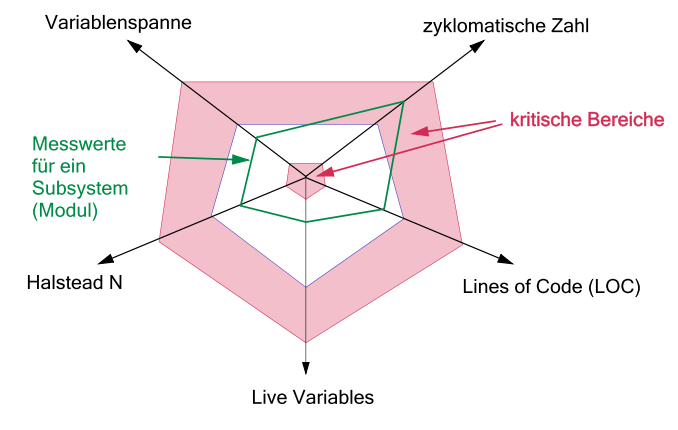
\includegraphics[width=0.85\textwidth]{3_1_3}
\end{figure}

\paragraph{Lines of Code = LOC}

LOC ist die naheliegendste Metrik. Festlegung des LOC:
\begin{itemize}
	\item Anzahl aller Zeilen der Textdatei(en) des betrachteten Programmteils
	\item Anzahl Zeilen der Textdatei(en) ohne Kommentare und Leerzeilen
	\item Anzahl Trennzeichen zwischen Anweisungen, also '';'' oder ...
	\item Anzahl Trennzeichen wie '';'' plus Schlüsselwörter wie ''IF'',...
	\item Knoten im Kontrollflussgraphen
	\item Programmlänge nach Halstead
\end{itemize}

\paragraph{LOC(Programmteil) = Anzahl der Knoten im Kontrollflussgraphen} 
Idee dieser Maßzahl:
\begin{itemize}
	\item betrachtete Programmteile oder ganze Programme mit hoher LOC sind zu komplex (no separation of concerns) und deshalb fehlerträchtig
	\item Programmteile mit geringer LOC sind zu klein und führen zu unnötigen Schnittstellenproblemen
\end{itemize}
Probleme mit dieser Maßzahl:
\begin{itemize}
	\item Kanten = Kontrollflusslogik spielen keine Rolle
	\item wie bewertet man geerbten Code einer Klasse
\end{itemize}

\paragraph{Zyklomatische Zahl(Komplexität) nach McCabe:}
\textbf{ZZ(Programmteil) = |E| - |N| + 2k} mit G als Kontrollflussgraph des Untersuchten Programmteils und
\begin{itemize}
	\item |E|:= Anzahl Kanten von G
	\item |N|:= Anzahl Knoten von G
	\item k:= Anzahl Zusammenhangskomponenten von G (Anzahl der nicht miteinander verbundenen Teilgraphen von G)
\end{itemize}

\textbf{Regel von McCabe:} ZZ eines in sich abgeschlossenen Teilprogramms (Zusammenhangskomponente) sollte nicht höher als 10 sein, da sonst Programm zu komplex und zu schwer zu testen ist

\paragraph{Interpretation und Probleme mit der zyklomatischen Zahl (Komplexität):}

\begin{itemize}
	\item es wird die Anzahl der Verzweigungen (unabhängigen Pfade) in einem Programm gemessen
	\begin{itemize}
		\item es wird davon ausgegangen, dass jede Zusammenhangskomponente (Teilprogramm) genau einen Eintritts- und einen Austrittsknoten hat
		\item damit besitzt jede Zusammenhangskomponente mit n Knoten mindestens n-1 Kanten; diese immer vorhandenen Kanten werden nicht mitgezählt
		\item die kleinste Komplexität einer Zusammenhangskomponente soll 1 sein, also wird von der Anzahl der Kanten n abgezogen und 2 addiert
	\end{itemize}
	\item in GOTO-freien Programmen wird damit genau die Anzahl der bedingten Anweisungen und Schleifen (if/while-Statements) gemessen
	\item die Zahl ändert sich nicht beim Einfügen normaler Anweisungen
	\item deshalb ist die Regel von McCabe mit \textbf{ZZ(Komponente) < 11} umstritten, da allenfalls eine Aussage über Testaufwand (Anzahl der zu testenden unabhängigen Programmpfade) getroffen wird
\end{itemize}

\paragraph{Halstead-Metriken - Eingangsgrößen:}

Die Halstead-Metriken messen verschiedene Eigenschaften einer Software-komponente. Als Eingabe dienen immer:
\begin{itemize}
	\item $\eta_{1}$: Anzahl der unterschiedlichen Operatoren eines Programms (verwendete arithmetische Operatoren, Prozeduren, Methoden, ... )
	\item $\eta_{2}$: Anzahl der unterschiedlichen Operanden eines Programms (verwendete Variablen, Parameter, Konstanten, ... )
	\item $N_{1}$: Gesamtzahl der verwendeten Operatoren in einem Programm (jede Verwendungsstelle wird separat gezählt)
	\item $N_{2}$:  Gesamtzahl der verwendeten Operanden in einem Programm (jede Verwendungsstelle wird separat gezählt)
	\item $\eta := \eta_{1}+\eta_{2}$:  Anzahl der verwendeten Deklarationen \textbf{(Programmvokabular)}
	\item $N := N_{1} + N_{2}$:Anzahl der angewandten Auftreten von Deklarationen (wird auch „normale“ Programmlänge genannt)
\end{itemize}

In der Literatur vorgeschlagene Zählregeln für Operatoren in Java:
\begin{itemize}
	\item Arithmetische und logische Standardoperatoren
	\item Sonderzweichen (Zuweisung, Konkatenation, Attributselektion)
	\item Reservierte Java-Schlüsselwörter
	\item Definitionen von Methoden und Funktionen
\end{itemize}

\paragraph{Halstead-Metriken - Definition:}
\begin{enumerate}
	\item \textbf{Berechnete Programmlänge} $L := \eta_{1}log_{2}\eta_{1} + \eta_{2}log_{2}\eta_{2}$ (hängt also nur von Anzahl verwendeter Operatoren und Operanden ab; postuliert wird, dass man  mit einer festen Anzahl von Operatoren und Operanden immer Programme einer bestimmten logischen Größe schreibt)
	\item \textbf{Programmgröße} $V=N log_{2} \eta$ (Programme Volume) (optimale Codierung des Programms als Bitvektor)
	\item ...
\end{enumerate}

\textbf{Bewertung:} Es gibt eine ganze Reihe weiterer Halstead-Metriken, deren Nutzen umstritten ist, und die versuchen zu bewerten:
\begin{itemize}
	\item \textbf{Schwierigkeit} der Erstellung eines Programms
	\item \textbf{Adäquatheit} einer bestimmten Programmiersprache für Problemstellung
	\item \textbf{Aufwand} für Erstellung eines Programms
\end{itemize}

\paragraph{''Live Variable''-Definition:}
Die \textbf{''Live Variables''}-Metrik berechnet für eine Programmkomponente die durchschnittliche Anzahl lebendiger Variablen dieser Komponente je Knoten des zugehörigen Kontrollflussgraphen; eine Variable ist dabei von ihrer ersten Definitionsstelle (vom Startknoten aus) bis zur letzten Definitions- oder Referenzierungsstelle (vor dem Endknoten) \textbf{lebendig}. 
\\
\\
\textbf{Zusammenfassung:} Live Variables einer Komponente ist durchschnittliche Anzahl lebendiger Variablen in einem Programm pro Zeile (Knoten im Kontrollflussgraphen). Eine Variable ist von ihrer ersten Definitionsstelle (vom Startknoten aus) bis zur letzten Definitions- oder Referenzierungsstelle (vor dem Endknoten) lebendig.

\paragraph{''Variablenspanne''-Definition:}

Die \textbf{''Variablenspannen''}-Metrik einer Programmkomponente berechnet die durchschnittliche Spanne zweier direkt aufeinander folgender definierender oder referenzierender Auftreten derselben Variable im zugehörigen Kontrollflussgraphen; die Spanne zweier Knoten in einem Kontrollflussgraphen entspricht der Länge des kürzesten Pfades (Anzahl Kanten dieses Pfades) zwischen diesen beiden Knoten.
\\
\\
\textbf{Zusammenfassung:} Variablenspanne einer Komponente ist die durchschnittliche Spanne zweier direkt aufeinander folgender definierender oder referenzierender Auftreten derselben Variable

\paragraph{Anmerkung zu Live Variables und Variablenspanne:}

Mit diesen beiden Metriken versucht man nicht die ''Kontrollflusskomplexität'' oder einfache Größe einer Softwarekomponente, sondern die Komplexität des Datenflusses zu bewerten (wieviele Variablen muss man wie lange beim Erstellen von Programmteilen oder beim Nachvollziehen des Programmablaufs ''im Kopf behalten'').

\paragraph{Überlegungen zu Metriken für objektorientierte Programme:}

Betrachtet wird oft Kopplung von Klassen = Benutzt-Beziehungen zwischen Klassen:
\begin{itemize}
	\item \textbf{geringer fan-out} (wenige auslaufende Benutzt-Beziehungen) ist positiv, da sich dann eine Klasse auf wenige andere Klassen abstützt
	\item \textbf{hoher fan-in} (viele einlaufende Benutzt-Beziehungen) ist positiv, da dann eine Klasse von vielen Klassen (wieder-)verwendet wird
	\item beides kann nicht maximiert werden, da über alle Klassen hinweg gilt: \textbf{Summe fan-in = Summe fan-out}
\end{itemize}
Eine Klasse A benutzt eine Klasse B, wenn:
\begin{itemize}
	\item in A ein Verweis auf Objekt der Klasse B verwendet wird
	\item in A eine Operation einen Parameter der Klasse B verwendet
	\item in A eine Operation der Klasse B aufgerufen wird
\end{itemize}
Gesucht werden Metriken, die neben der Kopplung von Klassen folgende Aspekte in Maßzahlen zusammenfassen:
\begin{itemize}
	\item die Methoden einer Klasse sollten \textbf{enge Bindung (high cohesion)} besitzen, also einem ähnlichen Zweck dienen (wie misst man das?)
	\item die Klassen einer Vererbungshierarchie sollten ebenfalls \textbf{enge Bindung} besitzen
	\item die in einem Modul bzw. Paket zusammengefassten Klassen oder die in einer Klasse zusammengefassten Methoden sollten \textbf{enge Bindung} besitzen
	\item Klassen in verschiedenen Modulen bzw. Paketen sollte lose gekoppelt sein (wie misst man das?) \textbf{(loose coupling)}
	\item Klassen und Module bzw. Pakete sollten ein Implementierungsgeheimnis verbergen \textbf{(data abstraction, encapsulation)} 
	\item ...
\end{itemize}

\paragraph{Bindungsmetriken - LOCOM (Low Cohesion Metric)}
Die Bindung der Methoden einer Klasse wird untersucht. Methoden sind eng miteinander gebunden, wenn sie auf viele gemeinsame Attribute oder Felder zugreifen. 
\\
\\

\textbf{LOCOM1}
\begin{itemize}
	\item P := Anzahl der Paare von Methoden ohne gemeinsame Attributzugriffe
	\item  := Anzahl der Paare von Methoden mit gemeinsamen Attributzugriffen
	\item LOCOM1 := if P>Q then P-Q else 0
	\item Gewünscht wird Wert von LOCOM1 nahe 0
\end{itemize}
\textbf{LOCOM2}
\begin{itemize}
\item m := Anzahl Methoden $m_{i}$ einer Klasse \\
$m(a_{i})$ := Anzahl Methoden die auf Attribut $a_{i}$ zugreifen
\item  n := Anzahl Attribute $a_{i}$ einer Klasse
\item LOCOM1 := 1 - (m($a_{1}$)+...+m($a_{n}$))/(m*n)
\item Gewünscht wird kleiner Wert von LOCOM2
\end{itemize}

\paragraph{Weitere Metriken}
\begin{itemize}
	\item \textbf{Afferent Coupling (Ca/AC)}: Die Anzahl der Klassen ausserhalb eines betrachteten Teilsystems (Kategorie), die von den Klassen innerhalb des Teilsystems abhängen
	\item \textbf{Efferent Coupling (Ce/EC):} Die Anzahl der Klassen innerhalb eines betrachteten Teilsystems (Kategorie), die von Klassen ausserhalb des betrachteten Teilsystems abhängen
	\item \textbf{Instabilität (I)}:   I = Ce / (Ce+Ca)
	\begin{itemize}
		\item I hat einen Wert zwischen 0 und 1, falls nicht Ce + Ca = 0 gilt mit 0 = max. stabil u. 1 = max. unstabil
		\item der Wert 1 besagt, dass Ca = 0 ist; das betrachtete Teilsystem exportiert also nichts nach außen (keine Klassen und deren Methoden) 
		\item der Wert 0 besagt, dass Ce = 0 ist; das betrachtete Teilsystem importiert also nichts von außen (keine Klassen und deren Methoden)
		\item Der ''undefinierte'' Fall Ca = 0 und Ce = 0 kann nur auf ein (sinnloses) isoliertes Teilsystem zutreffen, das weder importiert noch exportiert 
	\end{itemize}
	\item \textbf{Coupling als Change Dependency between Classes (CDBC)}. CDBC bewertet Aufwand, der mit Überarbeitung von CC wegen Änderung in SC verbunden sein könnte (Anzahl potentiell zu überarbeitender Methoden in CC).
	\begin{itemize}
		\item  n falls SC Oberklasse von CC ist (n = Anzahl Methoden in CC)
		\item n falls CC ein Attribut des Typs SC hat
		\item j falls SC in j Methoden von CC benutzt wird (als Typ lokaler Variable, Parameter oder Methodenaufruf von SC)
	\end{itemize}
	\item \textbf{Encapsulation als Attribute Hiding Factor (AHF)}.
	\begin{itemize}
		\item Sind alle Attribute als „private“ definiert, dann ist AHF = 1.
		\item Summe der Unsichtbarkeiten aller Attribute in allen Klassen geteilt durch die Anzahl aller Attribute
		\item Unsichtbarkeit eines Attributs := Prozentzahl der Klassen, für die das Attribut nicht sichtbar ist (abgesehen von eigener Klasse)
	\end{itemize}
	\item \textbf{Tiefe von Vererbungshierarchien:} zu tiefe Hierarchien werden unübersichtlich; man weiss nicht mehr, was man erbt
	\item \textbf{Breite von Vererbungshierarchien:} zu breite Vererbungshierarchien deuten auf Fehlen von zusammenfassenden Klassen hin
	\item \textbf{Anzahl Redefinitionen in einer Klassenhierarchie:} je mehr desto gefährlicher
	\item \textbf{Anzahl Zugriffe auf geerbte Attribute:} sind ebenfalls gefährlich, da beim Ändern von Attributen oder Attributzugriffen in Oberklasse die Zugriffen in den Unterklassen oft vergessen werden
\end{itemize}

\paragraph{Komplexitätsmaße:}
\begin{itemize}
	\item \textbf{Response for Class (RFC):}
	die Anzahl der in der Klasse deklarierten Methoden + die Anzahl der geerbten Methoden + die Anzahl sichtbarer Methoden anderer Klassen (Alle Methoden, die aufgerufen werden können? Sehr schwammig definiert!!!)
	\item \textbf{Weighted Methods Per Class (WMPC1):} \\
	die Summe der zyklomatischen Zahlen ZZ aller Methoden der Klasse (ohne geerbte Methoden)
	\item \textbf{Number of Remote Methods (NORM):}
	die Anzahl der in einer Klasse gerufenen Methoden ''fremder'' Klassen (also nicht die Klasse selbst oder eine ihrer Oberklassen)
	\item \textbf{Attribute Complexity (AC):}
	die gewichtete Summe der Attribute einer Klasse wird gebildet; Gewichte werden gemäß Typen/Klassen der Attribute vergeben. 
\end{itemize}


\subsection{Zusammenfassung}
Die \textbf{Visualisierung von Software} ist sowohl beim ''Forward Engineering'' für den Entwurf neuer Programmarchitekturen als auch beim „Reverse Engineering“ für das Studium von ''Legacy Software'' mit unbekannter Programmstruktur sehr hilfreich.
\\
\\
Werkzeugunterstützte \textbf{statische Analyseverfahren} helfen frühzeitig bei der Identifikation kritischer Programmstellen. Es sollten folgende Analyseverfahren immer eingesetzt werden:
\begin{itemize}
	\item \textbf{Stilanalyse} (Überprüfung vereinbarter Programmierkonventionen)
	\item \textbf{''dead code''-Analyse} (oft in Compiler eingebaut): nie verwendete Methoden, Variablen, Parameter, ... (wurde bisher nicht angesprochen)
	\item \textbf{Datenflussanalyse} (wenn Werkzeug verfügbar)
\end{itemize}
Weitere Analyseverfahren und vor allem \textbf{Metriken} sollten in großen Projekten zumindest versuchsweise eingesetzt werden.

\paragraph{Vorgehensweise beim Einsatz von Maßen}
\begin{enumerate}
	\item Fragen zur Ausgangssituation
	\begin{itemize}
		\item  In welcher Phase (Aktivitätsbereich) des Softwareentwicklungsprozesses soll eine Verbesserung eingeführt werden (z.B. Design, Codierung, ... )?
		\item Was soll damit erreicht werden bzw. welche Art von Fehler soll reduziert werden (z.B. Reduktion C++ Codierungsfehler)?
		\item Welche Methode soll eingesetzt werden (z.B. OO-Metriken)?
		\item Welche Technik/Werkzeug soll eingesetzt werden
	\end{itemize}
	\item \textbf{Bewertung des aktuellen Standes} des Entwicklungsprozesses:
	\begin{itemize}
		\item Welche Kosten u. welcher Aufwand entstehen  in welcher Phase?
		\item Wie ist die Qualität  der Ergebnisse jeder Phase?
		\item In welcher Phase entsteht welcher Anteil an Fehlern und welcher Teil der Fehlerbeseitigungskosten?
	\end{itemize}
	\item Mittel zur Bestimmung des aktuellen Standes, \textbf{zu messende Aspekte:}
	\begin{itemize}
		\item Kosten- und Zeitverfolgung beim Entwicklungsprozess
		\item  Definition von Qualitätsmaßen für Produkt pro Phase
		\item Erhebung von Fehlerstatistiken
	\end{itemize}
	\item \textbf{Analyse der Ergebnisse} und Erarbeitung von Verbesserungsvorschlägen:
	\begin{itemize}
		\item Auswertung der Maße
		\item Definition von Zielen auf Basis der Messwerte
		\item Entscheidung für Verbesserung in bestimmten Phasen
		\item Auswahl geeigneter Methoden und Werkzeuge
		\item Einführung der Methoden und Werkzeuge in Entwicklungsprozess
	\end{itemize}
	\item Bewertung der durchgeführten Änderungen:
	\begin{itemize}
		\item Kontinuierliche Weiterauswertung der Maße
		\item erneute Analyse nach ''Abklingen von Einschwingvorgängen''
	\end{itemize}
\end{enumerate}









